\chap{Experiments and Results}


\section{Introduction}

In this chapter, we look at the implementation perspective of the whole system. We also look at the three dataset we used and the results obtained from them. 

\section{Implementation Details}
To implement the conditional generative adversarial network we used Tensorflow\cite{tensorflow2015-whitepaper} with Kera\cite{keras}. The structure of generator and discriminator are described in \cref{Generator-Activation} and \cref{Discriminator-Table}.
\begin{table}[ht]
\centering
\caption{Generator Architecture Specification}
\label{Generator-Activation}
\begin{tabular}{llll}
Operation       & Stride & Features & Activation \\
Merge Input     & -      & -        & -          \\
Dense layer     & -      & -        & Sigmoid    \\
Deconvolution 1 & 5 * 5  & 512      & RELU       \\
Deconvolution 2 & 5 * 5    & 256      & RELU       \\
Deconvolution 3 & 5 * 5   & 128      & RELU       \\
Deconvolution 4 & 5 * 5   & 64       & RELU       \\
Deconvolution 5 & 5 * 5  & 3        & Tanh      
\end{tabular}
\end{table}
\begin{table}[ht]
\centering
\caption{Discriminator Architecture Specification}
\label{Discriminator-Table}
\begin{tabular}{llll}
Operation     & Stride & Features & Activation \\
Convolution 1 & 5 * 5  & 64       & Leaky RELU \\
Convolution 2 & 5*5    & 128      & LeakyRELU  \\
Convolution 3 & 5 *5   & 256      & LeakyRELU  \\
Convolution 4 & 5 *5   & 512      & LeakyRELU  \\
Convolution 5 & 5 * 5  & 1        & Softmax    \\
Convolution 5 & 5*5    & 18       & Sigmoid   
\end{tabular}
\end{table}
\section{Training}
Since the discriminator was weak, before actual training we trained the discriminator in two steps. Firstly we added a conditional vector to its input and removed the classification output of it. And we trained the discriminator with real images with incorrect label to classify as fake image. Secondly , to the original discriminator we copied the weights from the previous training and trained again on real images to classify the them into the particular class.  
\section{DataSet}
\subsection{CelebA}
The CelebFaces Attributes dataset (CelebA)\cite{celeba} contains 202599 face images of celebrities. As some of the categories are very less , so we removed certain categories from our training. . The sdistribution of the overall dataset is shown in \cref{fig:celeba}. As part of preprocessing, we crop the images to $64 \times 64$.The reason for cropping the images is to focus on faces in the images and as they are already aligned.


\begin{figure}[H]
  \centering
    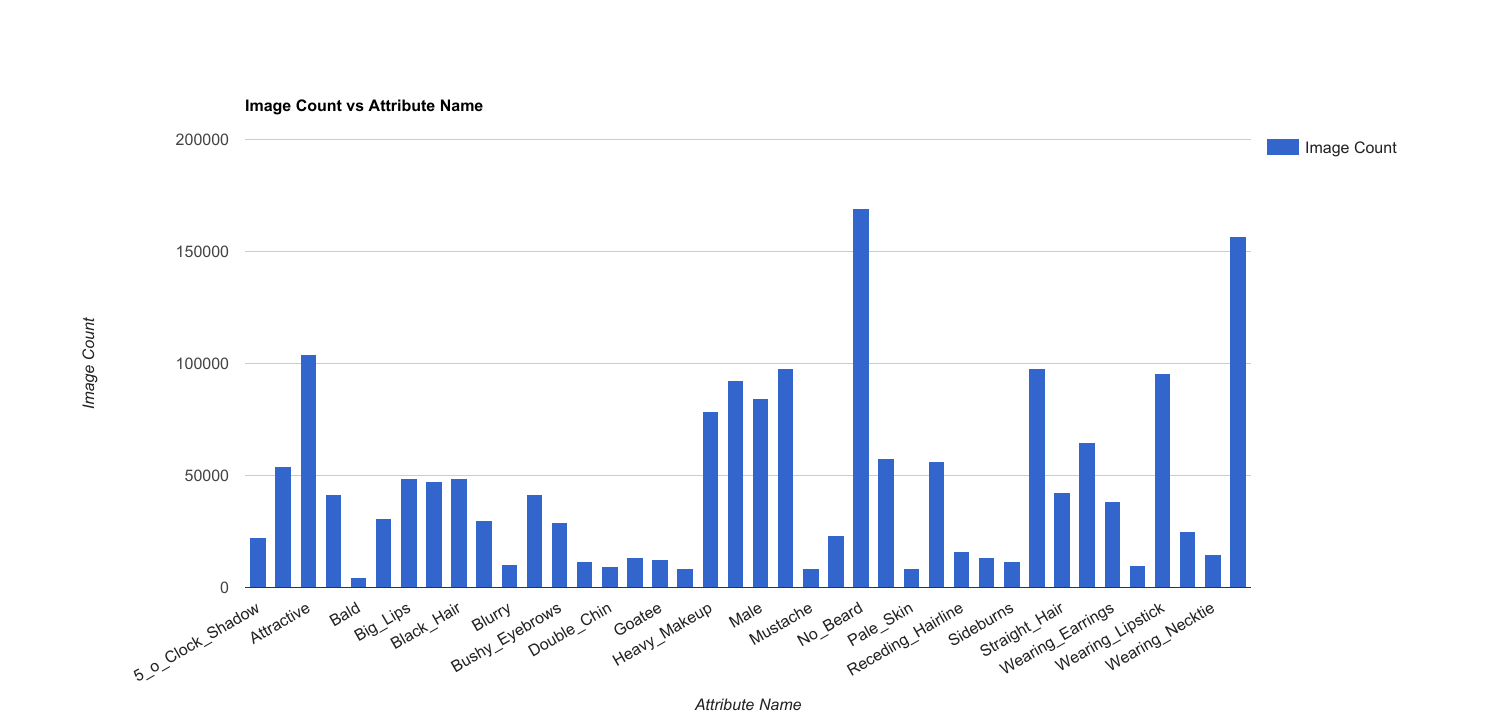
\includegraphics[scale=.3, angle=0]{Files/celeba-visualize.png}
    \caption[Generator Architecture]{Generator Architecture\cite{DCGAN}}
    \label{fig:celeba}
\end{figure}
\subsection{CIFAR-10}

\subsection{MNIST}
The MNIST dataset is very standard image processing dataset. This dataset contains xxx images of digits from 0 to 9. This dataset helps in validating the models correctness in very short time. Since neural  network take lot of time to converge, so if we have some issue with our implementation or logic then we can debug in very short amount of time.



\section{Evaluation}
It is very challenging to evaluate the performance of GAN networks. So, to evaluate and examine the performance we devised two methods. In the first method we will use the same discriminator to evaluate the accuracy of these images. Also to examine the over-fitting we look at the latent space.







